
\subsection{An explicit HOLD choice, tested prospectively}
The original controller did not separately learn whether to buy a merely reachable assessment. An additive supplement compares HOLD/continue-E against assessment jointly with price and reserves. It evaluates 108 development choices over 3,456 histories, freezes the choice, then runs 9,216 fresh histories: 4,608 selected-controller histories and 4,608 unchanged original-controller controls on the same fresh worlds. The three optional policies all select HOLD. This preserves the old results and leaves the operative configuration as E; it is not successful sharing.

The fresh reference mean E/HOLD profit is \$963.38750. Relative to the original sharing policy on those same fresh worlds, HOLD improves modeled mean net value by \$13.62320312, with conditional Monte Carlo 95\% interval [\$12.50606790, \$14.74033835]. This is avoided modeled assessment loss, not additional learned Alpha, new shared revenue or recovered historical profit. All 2,304 HOLD histories equal the corresponding E histories; 768 graph/library pairs match; the 2,304 unaffected control histories remain unchanged.
\begin{figure}[H]\centering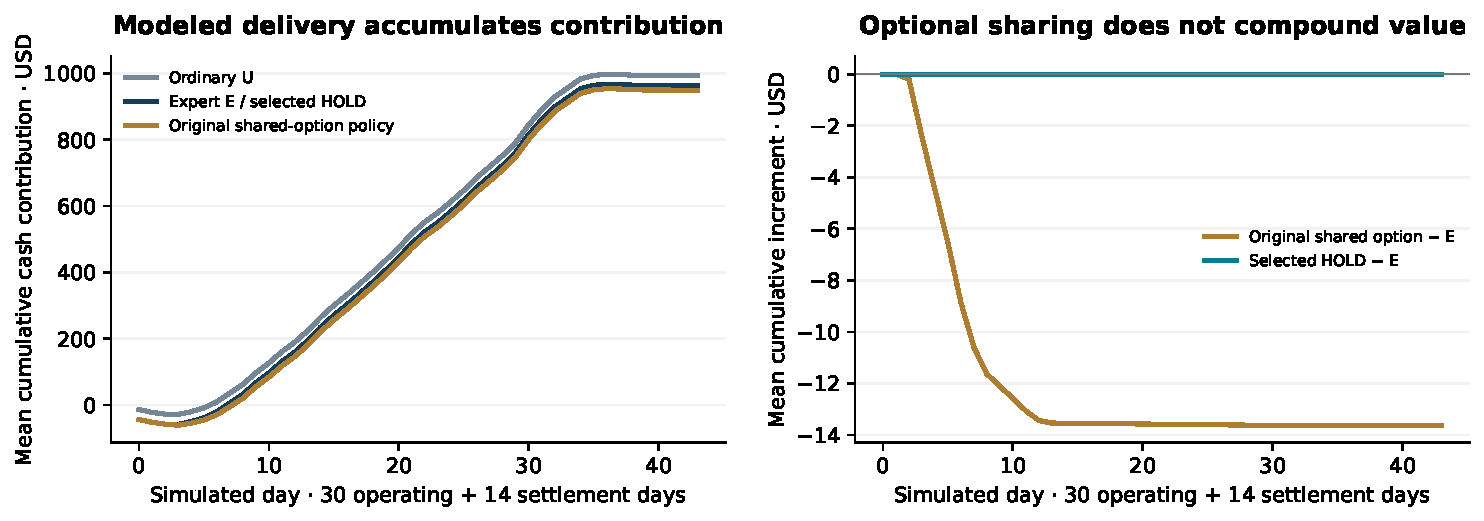
\includegraphics[width=0.97\linewidth]{figures/cumulative_value.pdf}\caption{Reconstructed from the retained fresh-reference event stream, 128 worlds per policy. All money is simulated; seed capital is excluded. The right panel isolates incremental net value rather than depicting more work as learning. HOLD equals E because it does not buy the uneconomic option under these assumptions.}\end{figure}
